\documentclass[border=4pt,12pt]{standalone}
% House style for redrawn exam diagrams (diagram-v4: 0.4pt lines, filled -latex arrows, fine dashes; stipple and hatching drawn as real dots/lines (no PDF/SVG patterns, so they render in every browser and at any scale); transparent background). Every figure \input's this.
\usepackage{amsmath,amssymb}
\usepackage{txfonts}
\usepackage{pdfrender,xcolor}
% \halo{text}: label on shading. The shading stops just around each letter's outline (a thin knock-out that follows the
% glyphs, like the papers' typesetting), never a box. Owner: "I don't want a box around the text".
\newcommand{\halo}[1]{\leavevmode\rlap{\pdfrender{TextRenderingMode=2,LineWidth=2.2pt,LineJoinStyle=1,StrokeColor=white,FillColor=white}#1}#1}
\usepackage{tikz,pgfplots}
\pgfplotsset{compat=1.18}
\usetikzlibrary{arrows.meta,calc,angles,quotes,patterns,patterns.meta,intersections,positioning,decorations.markings,shapes.geometric}
% Stipple and hatching are drawn as actual dots / lines clipped to the region (path picture), NOT as pattern fills:
% SVG <pattern> fills vanish or blur when browsers scale the image, so the owner could not see the shading.
% Each dot is a 0.72pt square (keeps SVGs small; reads as a dot at print size). Dots sit on one global staggered grid, so neighbouring regions line up.
\makeatletter
\newdimen\ex@x \newdimen\ex@y \newdimen\ex@xa \newdimen\ex@ya \newdimen\ex@xb \newdimen\ex@yb \newcount\ex@row
\def\exam@stipplecolor{black!75}\def\exam@dotr{0.42pt}\def\exam@dotgap{2.5}
\def\ex@rowdots{\ifdim\ex@x<\ex@xb \pgfpathrectangle{\pgfqpoint{\dimexpr\ex@x-0.36pt\relax}{\dimexpr\ex@y-0.36pt\relax}}{\pgfqpoint{0.72pt}{0.72pt}}\advance\ex@x by \exam@dotgap pt\relax\expandafter\ex@rowdots\fi}
\def\exam@stipple{%
  \pgftransformreset% dots are sized in real points even inside scaled pictures
  \pgfpointanchor{path picture bounding box}{south west}\ex@xa=\pgf@x \ex@ya=\pgf@y
  \pgfpointanchor{path picture bounding box}{north east}\ex@xb=\pgf@x \ex@yb=\pgf@y
  \pgfsetfillcolor{\exam@stipplecolor}\pgfmathsetmacro\ex@h{\exam@dotgap/2}%
  \pgfmathtruncatemacro\ex@r{floor(\ex@ya/\ex@h)-1}\ex@row=\ex@r\relax
  \ex@y=\ex@r\dimexpr\ex@h pt\relax
  \loop\ifdim\ex@y<\ex@yb
    \pgfmathtruncatemacro\ex@c{floor(\ex@xa/\exam@dotgap)-1}\ex@x=\ex@c\dimexpr\exam@dotgap pt\relax
    \ifodd\ex@row \advance\ex@x by \ex@h pt\fi
    \ex@rowdots
    \advance\ex@y by \ex@h pt \advance\ex@row by 1
    \ifnum\numexpr\ex@row-(\ex@row/4)*4\relax=0 \pgfusepath{fill}\fi% flush every 4 rows: bounded TeX memory, few clip copies in the SVG
  \repeat\pgfusepath{fill}}
\newdimen\ex@d
\def\exam@hatch#1{% #1 = 1 for /, -1 for \ ; lines 45 degrees, 3pt apart
  \pgftransformreset
  \pgfpointanchor{path picture bounding box}{south west}\ex@xa=\pgf@x \ex@ya=\pgf@y
  \pgfpointanchor{path picture bounding box}{north east}\ex@xb=\pgf@x \ex@yb=\pgf@y
  \ex@d=\dimexpr\ex@yb-\ex@ya\relax \ex@x=\dimexpr\ex@xa-\ex@d\relax
  \loop\ifdim\ex@x<\ex@xb
    \ifnum#1>0 \pgfpathmoveto{\pgfqpoint{\ex@x}{\ex@ya}}\pgfpathlineto{\pgfqpoint{\dimexpr\ex@x+\ex@d\relax}{\ex@yb}}%
    \else \pgfpathmoveto{\pgfqpoint{\ex@x}{\ex@yb}}\pgfpathlineto{\pgfqpoint{\dimexpr\ex@x+\ex@d\relax}{\ex@ya}}\fi
    \advance\ex@x by 4.24pt
  \repeat
  \pgfsetlinewidth{0.4pt}\pgfsetstrokecolor{black}\pgfusepath{stroke}}
\def\examstipple{\exam@stipple}\def\examhatch{\exam@hatch}\def\examsetstipplecolor#1{\def\exam@stipplecolor{#1}}\def\examsetdotgap#1{\def\exam@dotgap{#1}}
\makeatother
% (legacy pattern kept for old files)
% staggered stipple like the NESA papers' dotted shading
\pgfdeclarepatternformonly{exam stipple}{\pgfpointorigin}{\pgfqpoint{2.2pt}{2.2pt}}{\pgfqpoint{2.2pt}{2.2pt}}{%
  \pgfpathcircle{\pgfqpoint{0.55pt}{0.55pt}}{0.42pt}\pgfpathcircle{\pgfqpoint{1.65pt}{1.65pt}}{0.42pt}\pgfusepath{fill}}
\tikzset{
  every picture/.style={line width=0.6pt, >={Latex[length=2mm,width=1.3mm]}},
  curve/.style={line width=0.6pt},
  open arrow/.style={-{Latex[length=2mm,width=1.3mm]}},  % owner: filled -latex heads everywhere, no open chevrons
  aux/.style={dash pattern=on 2pt off 1.5pt, line width=0.6pt},
  shade/.code={\def\exA{#1}\def\exB{none}\ifx\exA\exB\else\pgfkeysalso{fill=black!18}\fi},
  shade/.default=on,
  shade dots/.style={fill=none, path picture={\examstipple}},
  stipple color/.code={\examsetstipplecolor{#1}},
  stipple gap/.code={\examsetdotgap{#1}},
  shade dense dots/.style={fill=none, stipple gap=1.6, path picture={\examstipple}},
  shade hatch/.style={fill=none, path picture={\examhatch{1}}},
  shade hatch reverse/.style={fill=none, path picture={\examhatch{-1}}},
  shade solid/.style={fill=black},
  pt/.style={circle, fill, inner sep=1.1pt},
  open pt/.style={circle, draw, fill=white, inner sep=1.1pt},
}
\pgfplotsset{
  exam axes/.style={axis lines=middle, axis line style={->}, xlabel={$x$}, ylabel={$y$},
    xlabel style={anchor=west}, ylabel style={anchor=south}, tick label style={font=\small},
    every axis plot/.append style={line width=0.6pt, black}, samples=200, clip=false,
    enlargelimits=false, axis on top},
}

\begin{document}
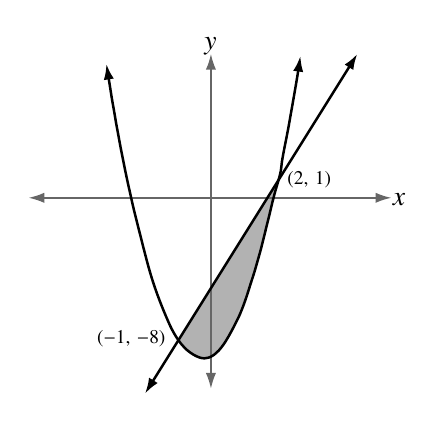
\begin{tikzpicture}[x=0.0127cm,y=-0.0127cm]
  % line y = 3x - 5: x = 342.5 - 0.625 (y - 60) in crop pixels
  \begin{scope}
    \clip (350,48) -- (137.5,388) -- (400,388) -- (400,48) -- cycle;
    \fill[black!30] plot[smooth] coordinates {(98.9,57.9) (100.8,70.01) (102.7,81.95) (104.6,93.89) (106.7,105.8) (108.7,117.6) (110.9,129.5) (113.1,141.4) (115.4,153.1) (117.8,165) (120.3,176.8) (122.9,188.4) (125.5,200.1) (128.4,211.8) (131.3,223.4) (134.3,235.3) (137.3,247) (140.3,258.4) (143.5,269.6) (147,280.5) (150.8,291.2) (155,302) (159.5,312.8) (164,322.7) (168.8,331.2) (174.1,338.6) (179.8,344.5) (186.1,349) (192.2,351.8) (197,352.6) (201.2,351.9) (206.1,349.4) (211.4,344.7) (216.5,338.2) (221.8,329.5) (227.2,319.4) (232,309.6) (236,299.7) (239.6,289.4) (243.2,278) (246.9,266.5) (250.1,255.4) (253.3,244) (256.2,232.5) (259.1,220.7) (262,209) (264.8,197.2) (267.7,186) (271,174.7) (273.3,165.6) (274.6,155.4) (276.5,144.8) (278.8,133.1) (281.1,121.2) (283.2,109.3) (285.3,97.42) (287.4,85.35) (289.4,73.59) (291.3,61.81) (293,50)};
  \end{scope}
  \draw[black!60,<->] (21,192) -- (384,192);
  \draw[black!60,<->] (203.5,383) -- (203.5,48);
  \node at (391,194) {$x$};
  \node at (203,40) {$y$};
  \draw[<->,line width=0.9pt] plot[smooth] coordinates {(98.9,57.9) (100.8,70.01) (102.7,81.95) (104.6,93.89) (106.7,105.8) (108.7,117.6) (110.9,129.5) (113.1,141.4) (115.4,153.1) (117.8,165) (120.3,176.8) (122.9,188.4) (125.5,200.1) (128.4,211.8) (131.3,223.4) (134.3,235.3) (137.3,247) (140.3,258.4) (143.5,269.6) (147,280.5) (150.8,291.2) (155,302) (159.5,312.8) (164,322.7) (168.8,331.2) (174.1,338.6) (179.8,344.5) (186.1,349) (192.2,351.8) (197,352.6) (201.2,351.9) (206.1,349.4) (211.4,344.7) (216.5,338.2) (221.8,329.5) (227.2,319.4) (232,309.6) (236,299.7) (239.6,289.4) (243.2,278) (246.9,266.5) (250.1,255.4) (253.3,244) (256.2,232.5) (259.1,220.7) (262,209) (264.8,197.2) (267.7,186) (271,174.7) (273.3,165.6) (274.6,155.4) (276.5,144.8) (278.8,133.1) (281.1,121.2) (283.2,109.3) (285.3,97.42) (287.4,85.35) (289.4,73.59) (291.3,61.81) (293,50)};
  \draw[<->,line width=0.9pt] (137.5,388) -- (350,48);
  \node[font=\scriptsize,anchor=west] at (270,174) {$(2,\,1)$};
  \node[font=\scriptsize,anchor=east] at (168,333) {$(-1,\,-8)$};
\end{tikzpicture}
\end{document}
